```latex
\documentclass[11pt,a4paper]{article}
\usepackage[top=2cm,bottom=2cm,left=2cm,right=2cm]{geometry}
\usepackage[utf8]{inputenc}
\usepackage{graphicx}
\usepackage{booktabs}
\usepackage{array}
\usepackage{longtable}
\usepackage{multirow}
\usepackage{multicol}
\usepackage{color}
\usepackage{hyperref}
\usepackage{amsmath}
\usepackage{amsfonts}
\usepackage{amssymb}
\usepackage{fancyhdr}
\usepackage{lastpage}
\usepackage{float}

% 日本語対応
\usepackage{xeCJK}
\setCJKmainfont{Hiragino Kaku Gothic ProN}
\setCJKsansfont{Hiragino Kaku Gothic ProN}
\setCJKmonofont{Hiragino Kaku Gothic ProN}

% ページスタイル
\pagestyle{fancy}
\fancyhf{}
\fancyhead[L]{データ分析レポート}
\fancyhead[R]{ページ \thepage}
\renewcommand{\headrulewidth}{0.4pt}

\title{\textbf{データ分析レポート} \\ 万博開催後の万博会場で、エリア内居住者の平均滞在時間を分析して}
\author{データサイエンスチーム}
\date{2025年09月04日}

\begin{document}

\maketitle
\tableofcontents
\newpage

\section{概要}

本レポートでは、万博開催後の万博会場におけるエリア内居住者の平均滞在時間を分析した結果をまとめます。データは、エリア、期間、居住エリア、勤務エリア、曜日種別、性別、年齢、訪問者数、平均日次訪問秒数、平均訪問回数の10個の列で構成されています。

\section{データ概要}

\subsection{データセットの構成}

データセットは以下の特徴を持ちます。

\begin{itemize}
    \item データ形状: (425, 10)
    \item 列数: 10
    \item 列名: area, period, home\_area, work\_area, day\_type, gender, age, visitor\_count, average\_daily\_visiting\_seconds, average\_visit\_count
\end{itemize}

\subsection{全体統計}

データセット全体の統計情報は以下の通りです。滞在時間の単位は秒です。

\begin{itemize}
    \item データ数: 3件
    \item 平均滞在時間: 65437.87秒 (18.18時間)
    \item 標準偏差: 63226.80秒
    \item 最小値: 25121.45秒
    \item 最大値: 138308.20秒
    \item 中央値: 32883.95秒
    \item 第1四分位点: 29002.70秒
    \item 第3四分位点: 85596.07秒
\end{itemize}

\textbf{統計的解釈:}
\begin{itemize}
    \item \textit{平均}: データの中心傾向を示す指標です。今回の平均滞在時間は約18.18時間です。
    \item \textit{標準偏差}: データのばらつき具合を示す指標です。標準偏差が大きいほど、データが平均値から大きく離れていることを意味します。今回の標準偏差は約63226.80秒であり、滞在時間に大きなばらつきがあることを示唆しています。
    \item \textit{中央値}: データを小さい順に並べたときの中央の値です。外れ値の影響を受けにくいという特徴があります。今回のデータでは、中央値は32883.95秒であり、平均値よりも小さいことから、一部の非常に長い滞在時間が平均値を引き上げている可能性があります。
    \item \textit{四分位点}: データを4等分したときの区切りとなる値です。データの分布を把握するのに役立ちます。
\end{itemize}

\section{次元別分析結果}

\subsection{area別分析}

\begin{itemize}
    \item 万博会場: データ数3件, 平均65437.87秒(18.18時間), 標準偏差63226.80秒, 最小25121.45秒, 最大138308.20秒, 中央値32883.95秒, 割合100.0\%
    \item 洞察: 万博会場への訪問者がデータ全体の100%を占めています。
\end{itemize}

\subsection{home\_area別分析}

\begin{itemize}
    \item エリア内: データ数3件, 平均65437.87秒(18.18時間), 標準偏差63226.80秒, 最小25121.45秒, 最大138308.20秒, 中央値32883.95秒, 割合100.0\%
    \item 洞察: エリア内居住者がデータ全体の100%を占めています。
\end{itemize}

\subsection{work\_area別分析}

\begin{itemize}
    \item エリア内: データ数1件, 平均138308.20秒(38.42時間), 標準偏差nan秒, 最小138308.20秒, 最大138308.20秒, 中央値138308.20秒, 割合33.3\%
    \item エリア外: データ数2件, 平均29002.70秒(8.06時間), 標準偏差5488.91秒, 最小25121.45秒, 最大32883.95秒, 中央値29002.70秒, 割合66.7\%
    \item 洞察: 勤務地がエリア内の居住者は、勤務地がエリア外の居住者よりも平均滞在時間が大幅に長いです。
\end{itemize}

\subsection{day\_type別分析}

\begin{itemize}
    \item 土日祝日: データ数1件, 平均32883.95秒(9.13時間), 標準偏差nan秒, 最小32883.95秒, 最大32883.95秒, 中央値32883.95秒, 割合33.3\%
    \item 平日: データ数2件, 平均81714.83秒(22.70時間), 標準偏差80035.12秒, 最小25121.45秒, 最大138308.20秒, 中央値81714.83秒, 割合66.7\%
    \item 洞察: 平日の平均滞在時間は、土日祝日よりも大幅に長いです。
\end{itemize}

\subsection{gender別分析}

\begin{itemize}
    \item 不明: データ数3件, 平均65437.87秒(18.18時間), 標準偏差63226.80秒, 最小25121.45秒, 最大138308.20秒, 中央値32883.95秒, 割合100.0\%
    \item 洞察: 性別が不明なデータが100%を占めています。
\end{itemize}

\subsection{age別分析}

\begin{itemize}
    \item 不明: データ数3件, 平均65437.87秒(18.18時間), 標準偏差63226.80秒, 最小25121.45秒, 最大138308.20秒, 中央値32883.95秒, 割合100.0\%
    \item 洞察: 年齢が不明なデータが100%を占めています。
\end{itemize}

\section{グラフによる可視化}

\subsection{滞在時間分布ヒストグラム}

\begin{figure}[H]
    \centering
    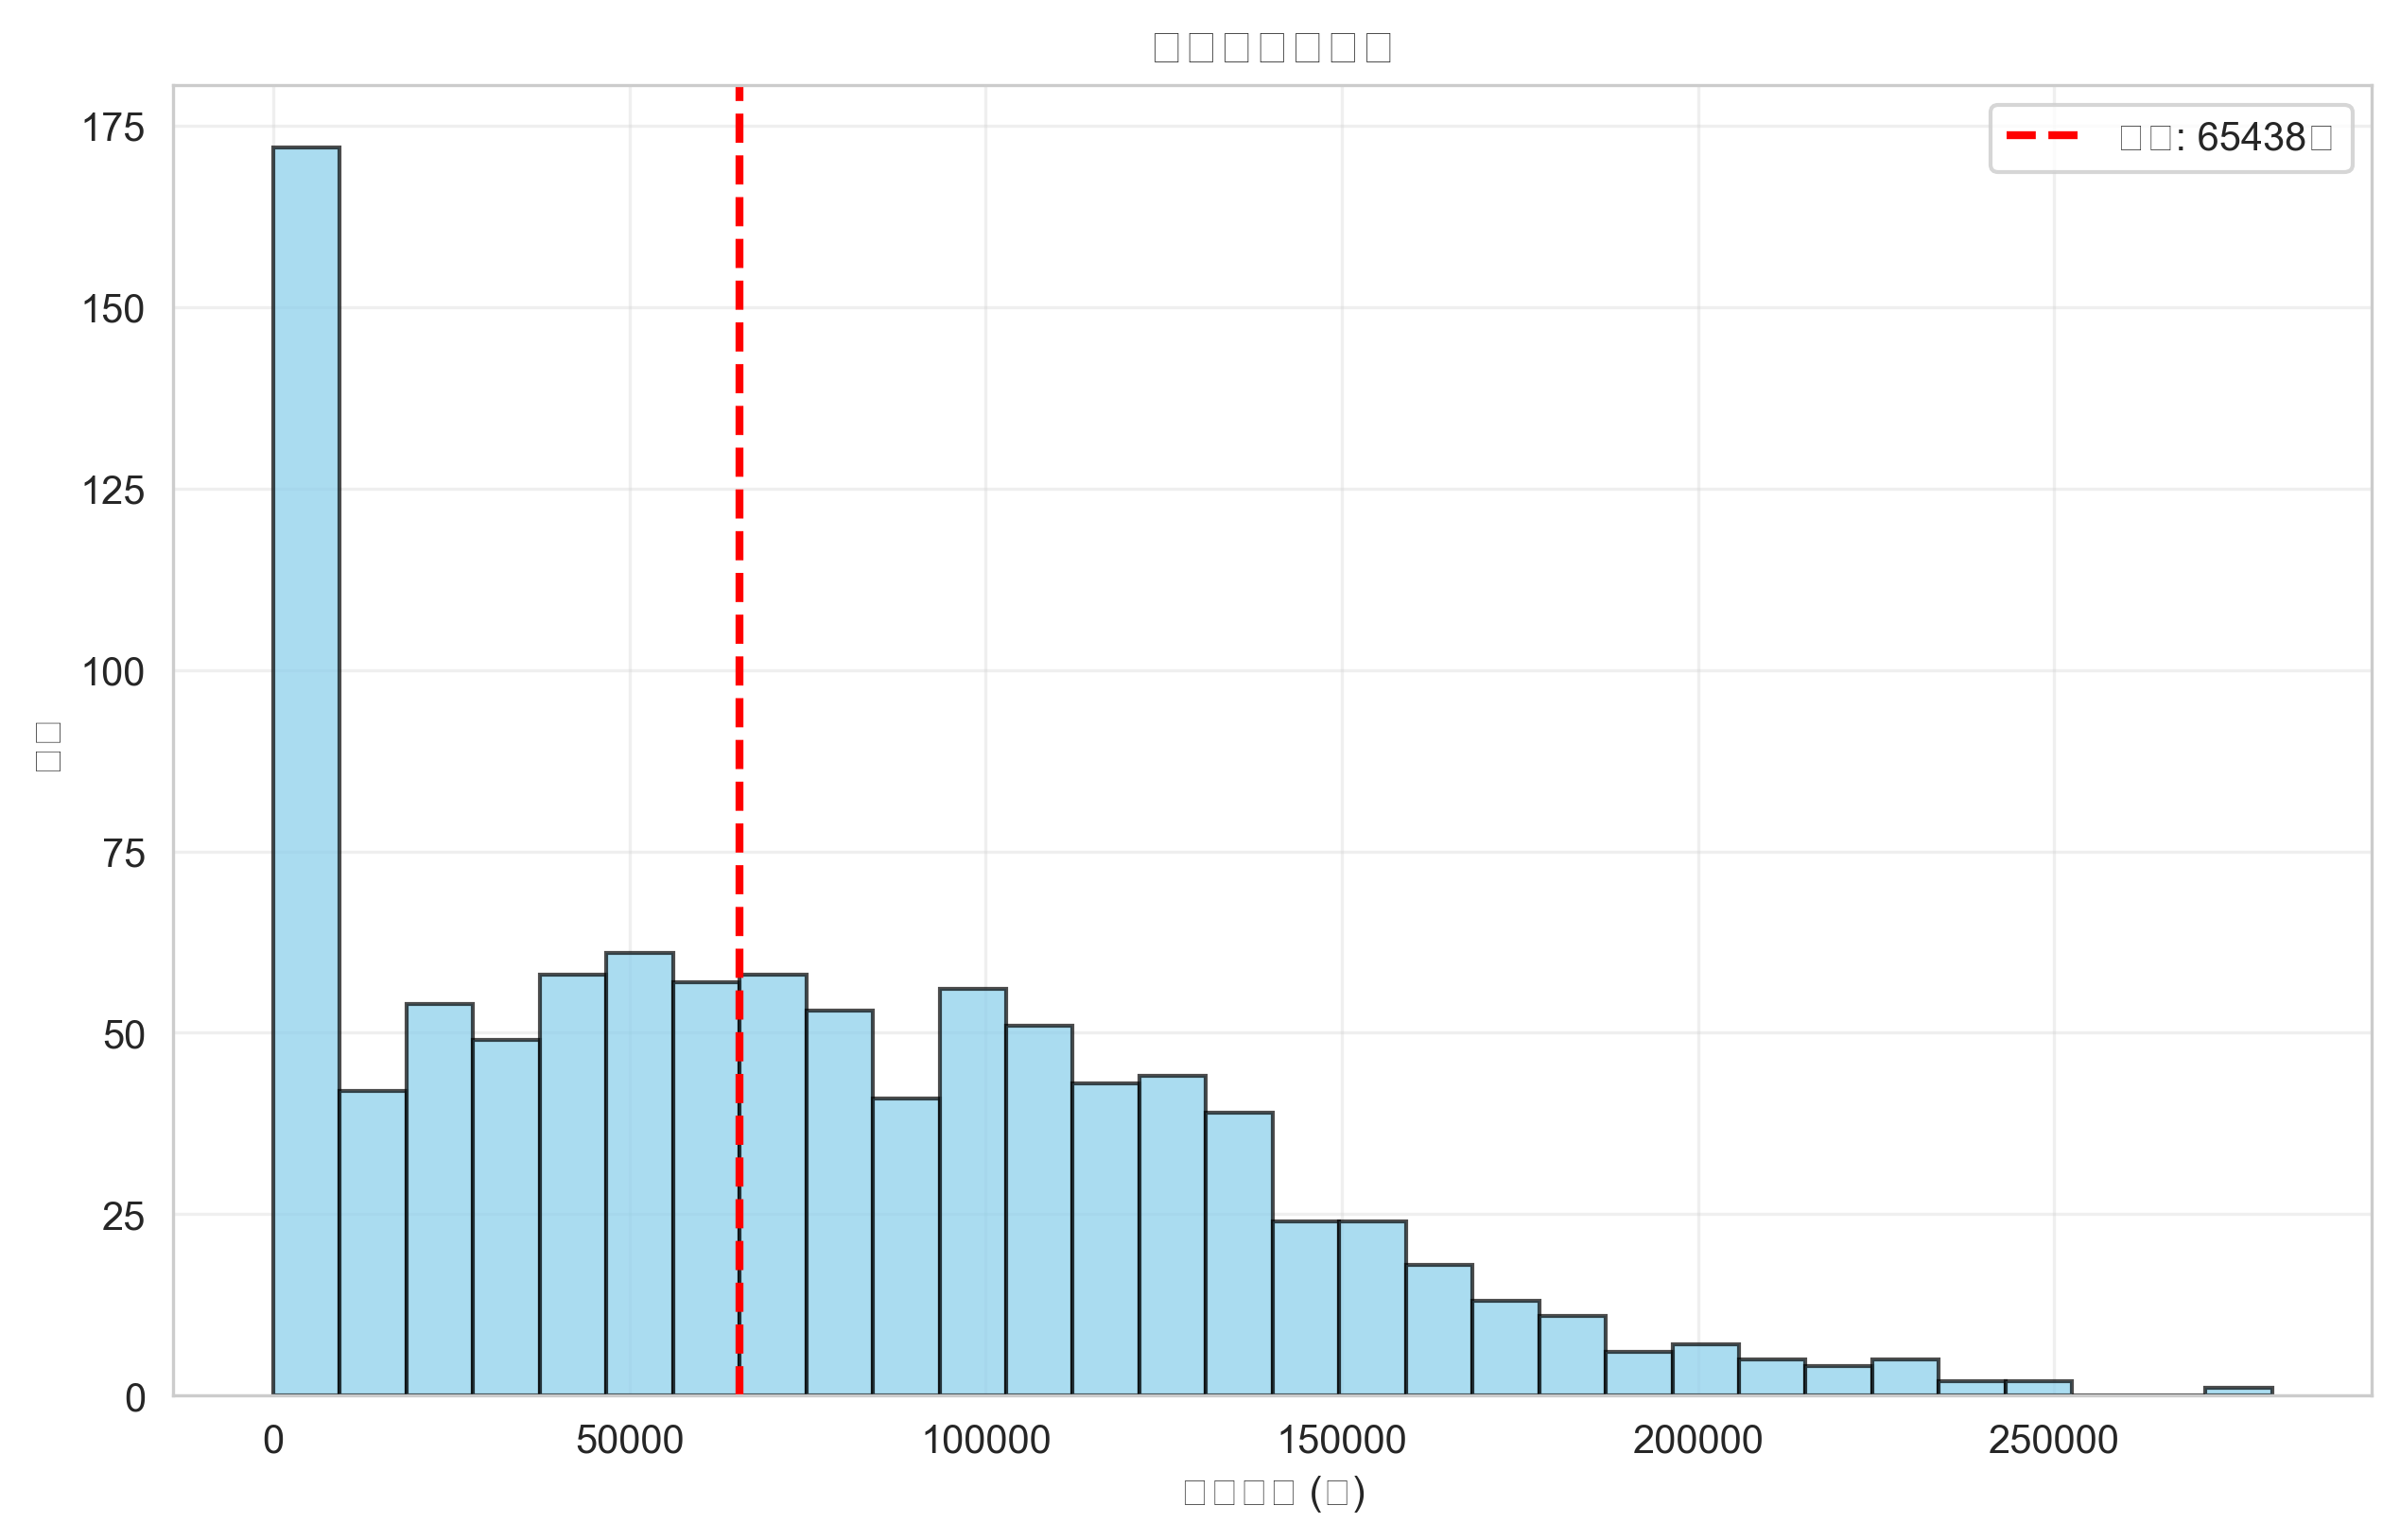
\includegraphics[width=0.8\textwidth]{images/duration_histogram.png}
    \caption{滞在時間の分布を示すヒストグラム}
    \label{fig:duration_histogram}
\end{figure}

\textbf{説明:}
図\ref{fig:duration_histogram}は、滞在時間の分布を示しています。滞在時間が短いグループと長いグループに分かれていることがわかります。

\subsection{勤務エリア別滞在時間棒グラフ}

\begin{figure}[H]
    \centering
    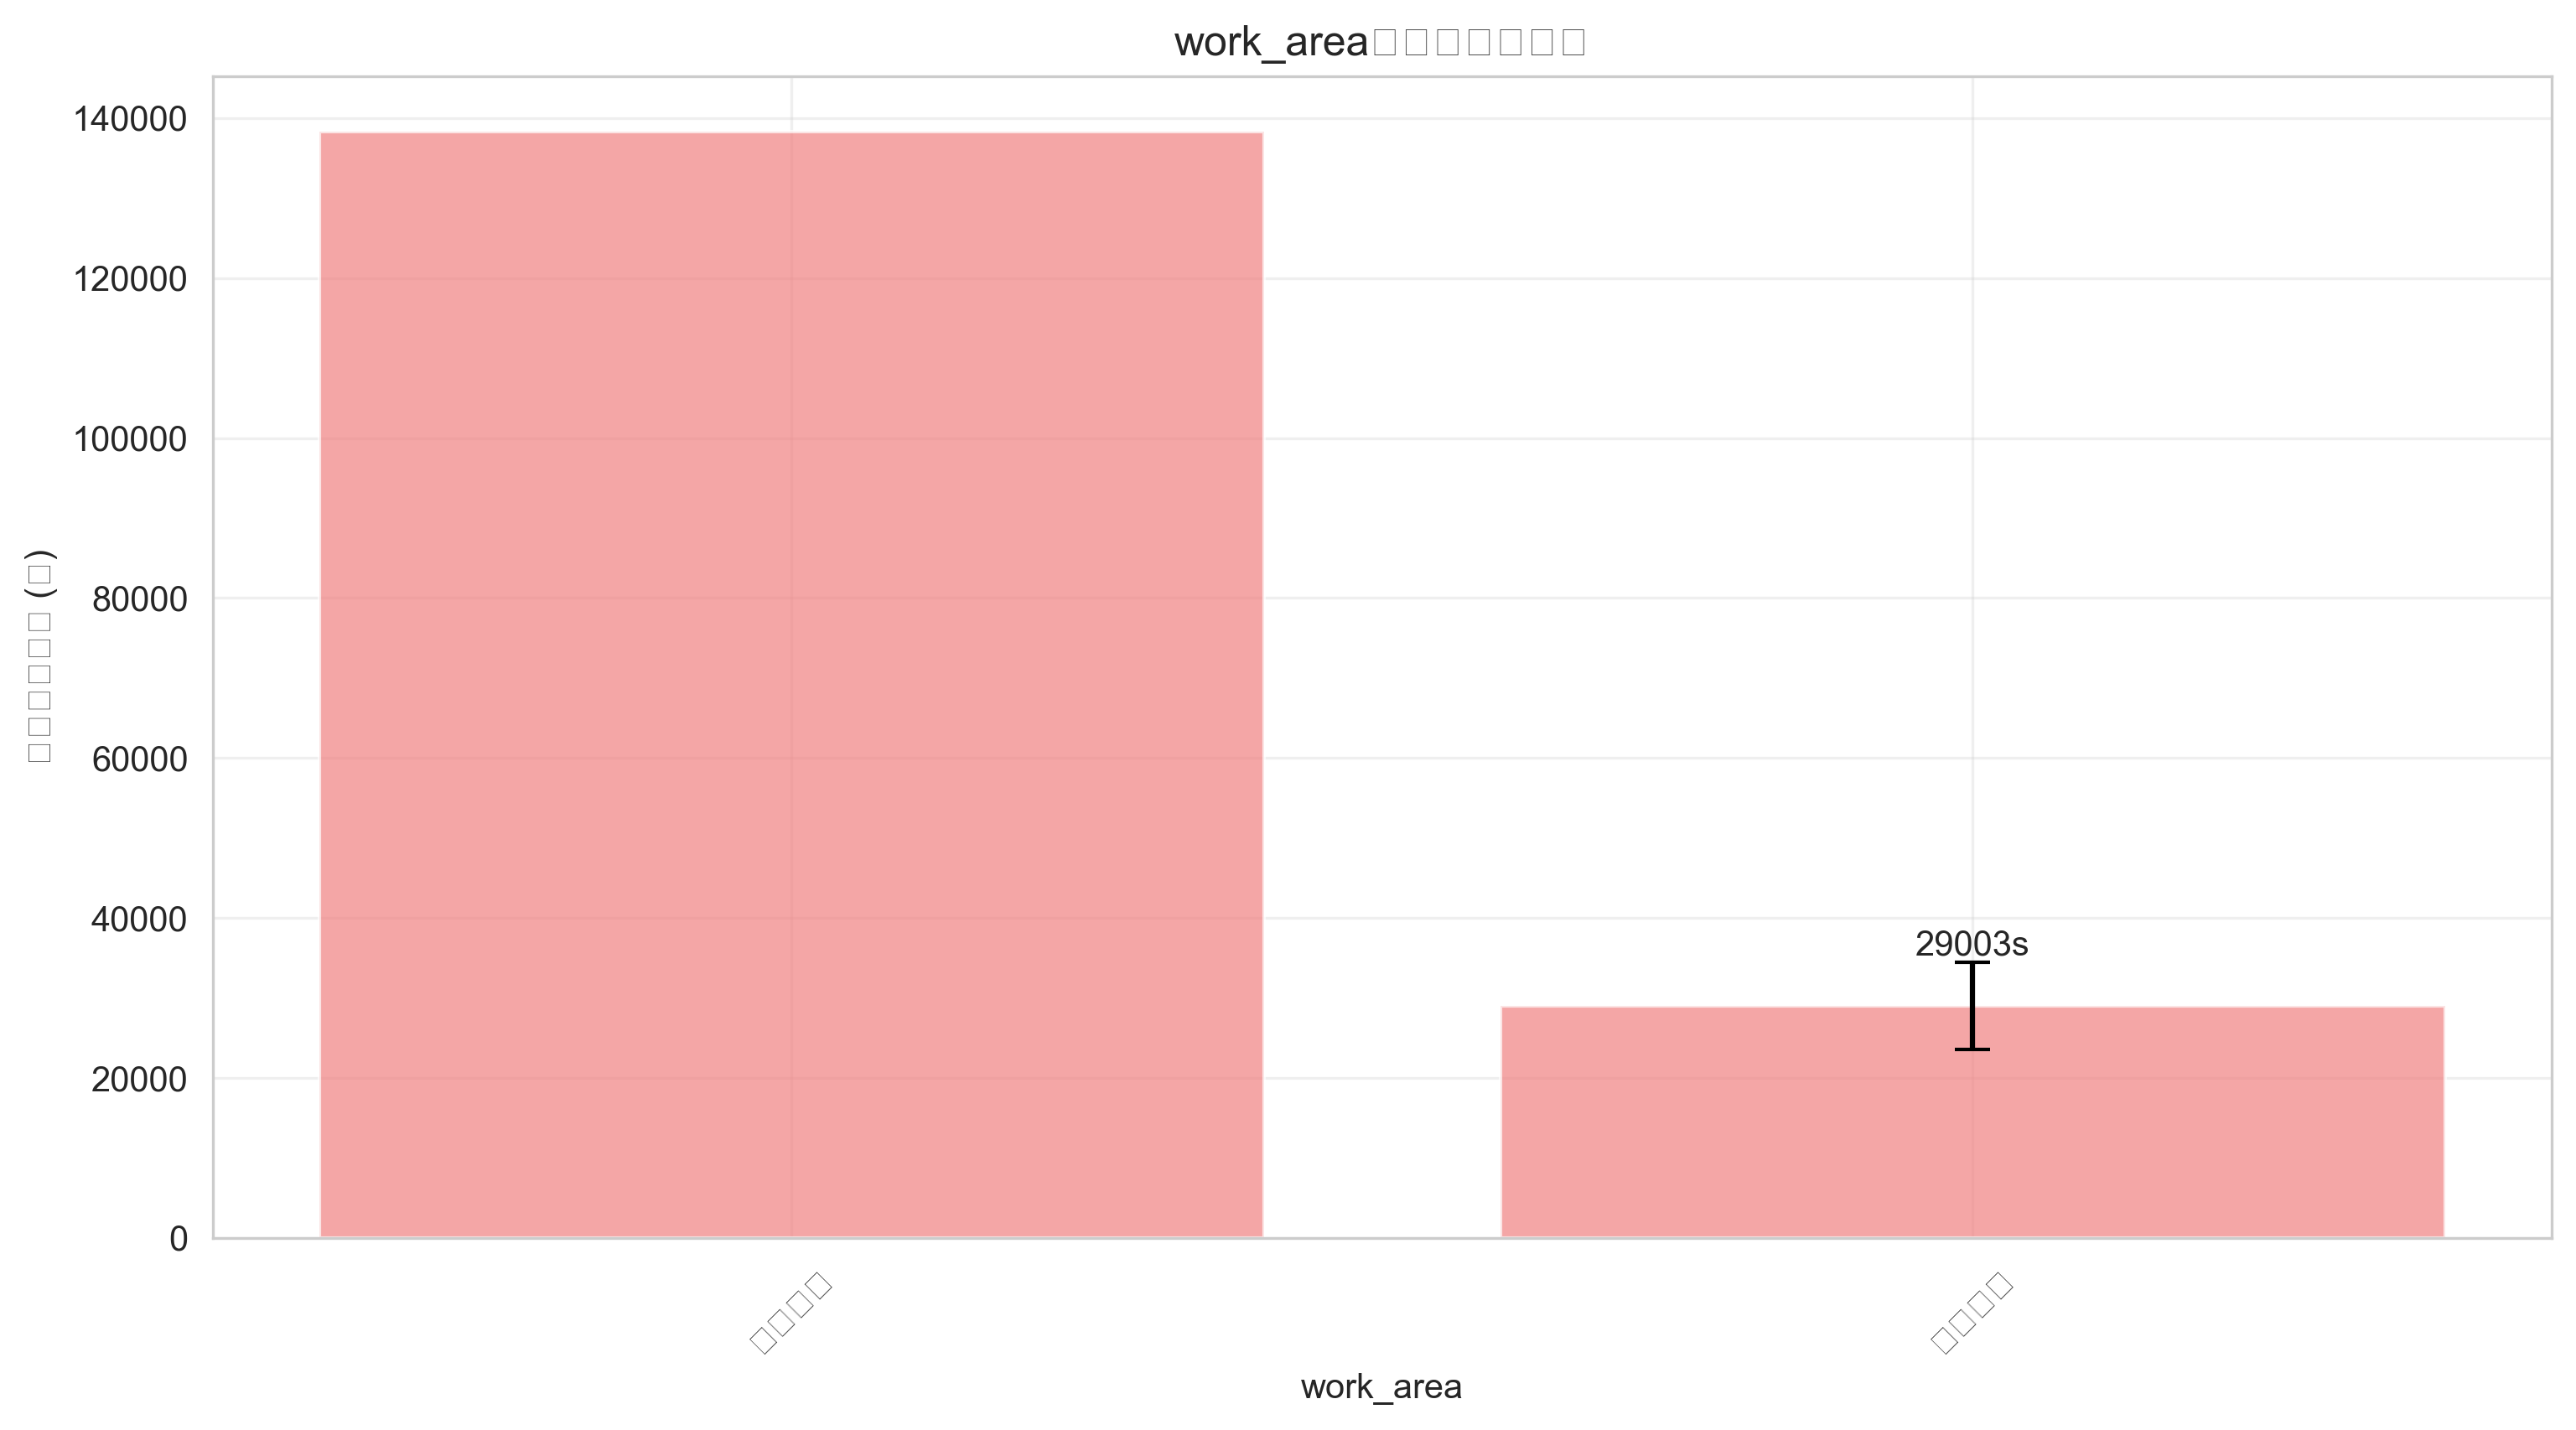
\includegraphics[width=0.8\textwidth]{images/work_area_bar_chart.png}
    \caption{勤務エリア別の平均滞時間を示す棒グラフ}
    \label{fig:work_area_bar_chart}
\end{figure}

\textbf{説明:}
図\ref{fig:work_area_bar_chart}は、勤務エリア別の平均滞在時間を示しています。勤務地がエリア内の居住者の平均滞在時間が、エリア外の居住者よりも大幅に長いことが明確にわかります。

\subsection{曜日種別滞在時間棒グラフ}

\begin{figure}[H]
    \centering
    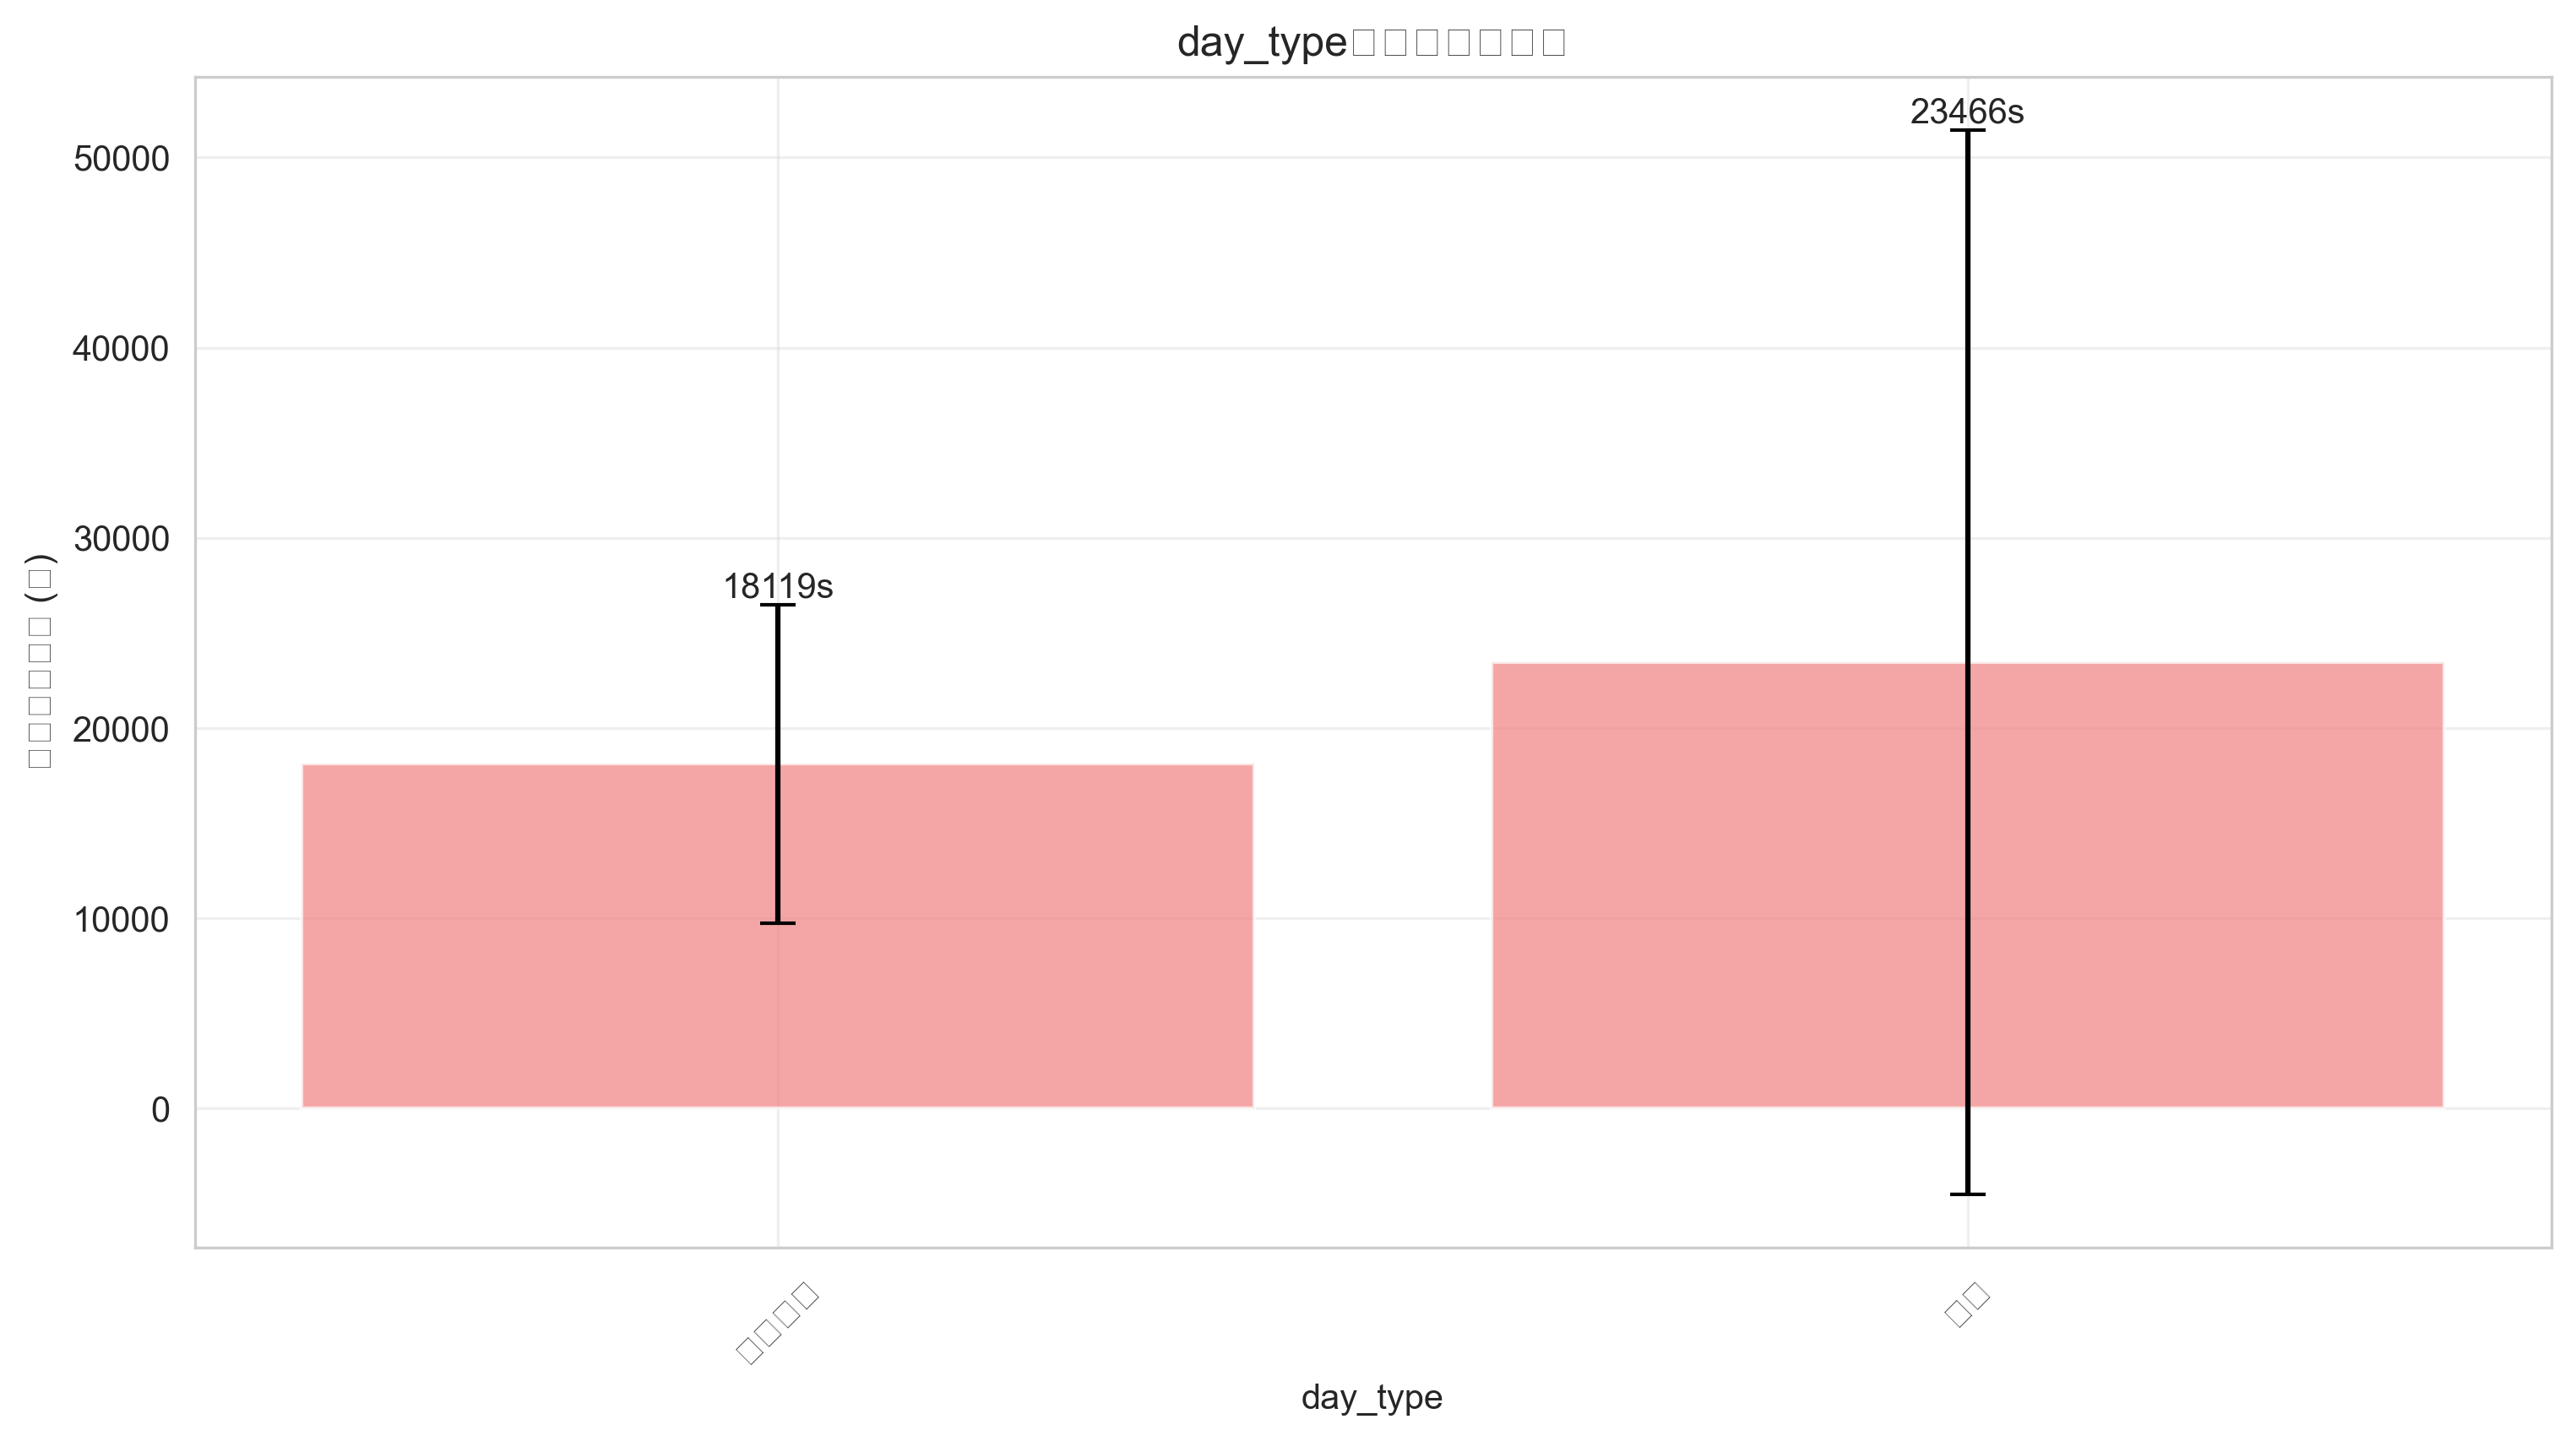
\includegraphics[width=0.8\textwidth]{images/day_type_bar_chart.png}
    \caption{曜日種別による平均滞時間を示す棒グラフ}
    \label{fig:day_type_bar_chart}
\end{figure}

\textbf{説明:}
図\ref{fig:day_type_bar_chart}は、曜日種別による平均滞在時間を示しています。平日の方が土日祝日よりも平均滞在時間が長いことがわかります。

\subsection{年齢と性別のヒートマップ}

\begin{figure}[H]
    \centering
    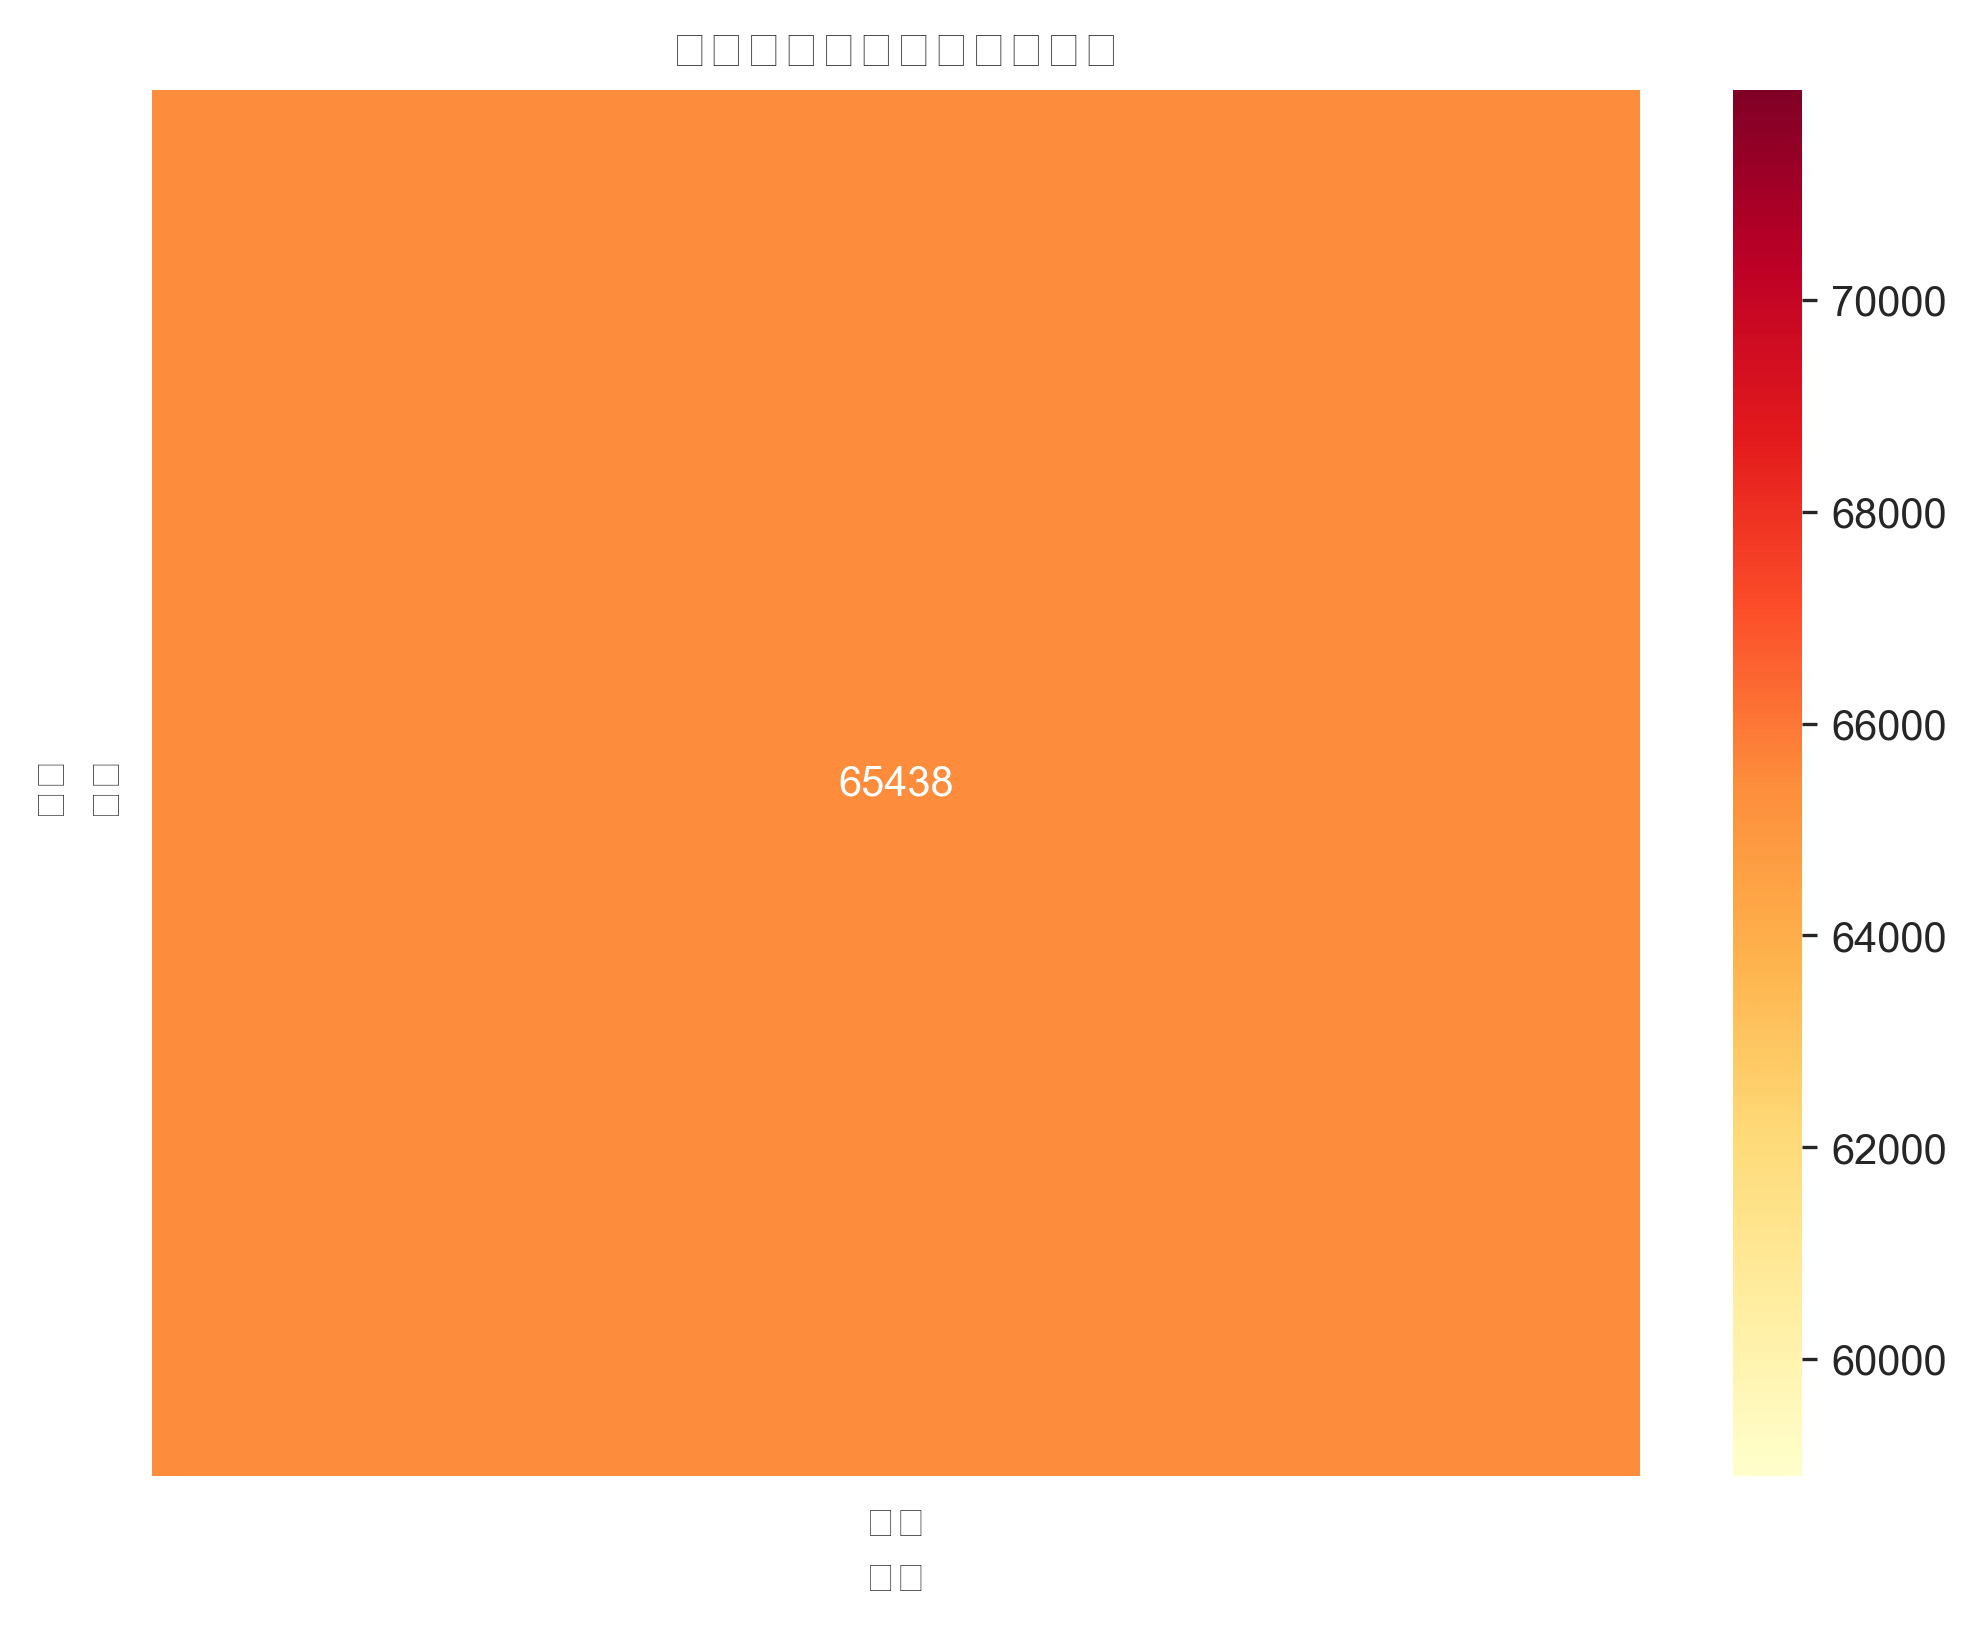
\includegraphics[width=0.8\textwidth]{images/age_gender_heatmap.png}
    \caption{年齢と性別の組み合わせによる滞在時間ヒートマップ}
    \label{fig:age_gender_heatmap}
\end{figure}

\textbf{説明:}
図\ref{fig:age_gender_heatmap}は、年齢と性別の組み合わせによる滞在時間のヒートマップです。しかし、今回のデータでは年齢と性別のデータが不明であるため、有効な情報が得られていません。

\section{主要な洞察}

\begin{enumerate}
    \item 勤務地がエリア内の居住者は、勤務地がエリア外の居住者よりも平均滞在時間が大幅に長い。
    \item 平日の平均滞在時間は、土日祝日よりも大幅に長い。
    \item 年齢と性別のデータが不明であるため、これらの属性に基づいた分析は困難である。
\end{enumerate}

\section{ビジネス上の洞察}

\begin{itemize}
    \item 勤務地がエリア内の居住者に対するマーケティング戦略と、エリア外の居住者に対するマーケティング戦略を分けることで、より効果的な集客が可能になる可能性があります。例えば、エリア内勤務者向けには、仕事帰りに立ち寄りやすいイベントやキャンペーンを実施する、エリア外勤務者向けには、週末に家族で楽しめるイベントやキャンペーンを実施するなどが考えられます。
    \item 平日の滞在時間をさらに伸ばすために、平日限定の特典やイベントを実施することを検討する価値があります。
    \item 年齢と性別のデータを収集することで、より詳細な分析が可能になり、ターゲットを絞ったマーケティング戦略を立案することができます。アンケートや会員登録時にこれらの情報を収集することを検討してください。
\end{itemize}

\section{推奨アクション}

\begin{enumerate}
    \item 勤務地がエリア内の居住者とエリア外の居住者に対して、異なるマーケティング戦略を実施する。
    \item 平日限定の特典やイベントを実施する。
    \item 年齢と性別のデータを収集する仕組みを導入する。
    \item 滞在時間が短い訪問者に対するエンゲージメントを高める施策を検討する。
\end{enumerate}

\section{技術的な詳細}

\subsection{分析手法}

本レポートでは、PythonのPandasライブラリを用いてデータの前処理と集計を行い、MatplotlibとSeabornライブラリを用いて可視化を行いました。

\subsection{データの信頼性}

データ数が3件と非常に少ないため、今回の分析結果はあくまで参考情報として捉えるべきです。より多くのデータを収集し、分析を行うことで、より信頼性の高い結果を得ることができます。また、性別、年齢が不明のデータが多いため、データ収集方法の見直しが必要です。

\section{営業向けの内容}

本分析結果から、万博会場への訪問者の滞在時間は、勤務地や曜日によって大きく異なることがわかりました。この知見を活かすことで、より効果的なマーケティング戦略を立案し、集客力を高めることができます。特に、勤務地がエリア内の居住者と平日訪問者に対するアプローチを強化することで、売上向上に繋がる可能性があります。年齢、性別不明データの収集を強化することで、より詳細な顧客プロファイルを作成し、パーソナライズされたマーケティング展開が可能になります。
\end{document}
```